\section{Evaluation}
\label{sec.evaluation}

In seeking to evaluate the performance of Lind, 
we designed and conducted a set of experiments based around four fundamental questions:

\begin{itemize}
\item Q1: What are the benefits of running applications in Lind, 
and not in other existing virtualization systems? (\S{\ref{Linux-Kernel-Bug-Test-and-Evaluation}})

\item Q2: Why is Lind less likely to trigger kernel bugs compared to 
other virtualization systems? (\S{\ref{Reachable-Kernel-Trace-Analysis-for-Different-Virtualization-Systems}})

\item Q3: Is Lind really secure? What happens if one of the building blocks of Lind, 
the Repy sandbox kernel has bugs? (\S{\ref{Reachable-Kernel-Trace-Analysis-for-Repy-Sandbox}})

\item Q4: Is Lind a practical tool that can run real-world applications at reasonable overhead? 
(\S{\ref{Performance-Evaluation}})
\end{itemize}

In this section, we describe the experiments designed to answer these question, 
and discuss how the results support the merits of our secure design and its prototype Lind. 

\subsection{Evaluation Methodology}

Our evaluation strategy was to directly compare the performance of Lind against 
four other existing virtualization systems\textendash VirtualBox, VMWare Workstation, 
Docker, and Graphene. We also compared it against Native Linux and used 
those results as a baseline for evaluation. Because Native Linux is the original OS, 
without virtualization and additional protection, this data helps to clarify the security benefits of Lind, 
as well as whatever performance overhead costs the system may incur.

\textbf{Experimental Setup:}

We conducted our experiments under Linux kernel 3.14.1, using the following protocols:

\begin{itemize}
\item We identified and examined a list of  69 historical bugs that have specifically 
targeted Linux kernel 3.14.1 \cite{CVE-Datasource}. Through analyzing security kernel patches for those bugs, 
we identified the lines of code in the kernel that correspond to each of one.

\item In order to test if a bug is triggerable, we created or located C code to 
exploit each of the kernel bugs \cite{Exploit-Database}. We were able to run and obtain results for 
35 out of the 69 bugs in our experiments. For the rest of the bugs, 
we could not find exploit code that would trigger them effectively at that moment. 
In addition, it was very difficult to accurately determine if more complex bugs 
were triggered or not. We leave further study and analysis of those bugs to future work.

\item We compiled and ran the exploit C code under each virtualization system to 
obtain their kernel traces, and then used our kernel trace safety metric to determine 
if a specific bug was triggered inside that virtualization system. 

\item Lastly, to  analyze the reachable kernel paths for each of the virtualization systems, 
we conducted system call fuzzing (similar to what we did in �3) to obtain the kernel trace in each system. 
We repeated the system call fuzzing within Repy as well to obtain its kernel trace. 
\end{itemize}

\subsection{Comparison Results and Analysis}

Since our primary goal was to build a secure system, our core evaluation was conducted primarily 
from a security perspective (\S{\ref{Linux-Kernel-Bug-Test-and-Evaluation}}, 
\S{\ref{Reachable-Kernel-Trace-Analysis-for-Different-Virtualization-Systems}}, 
\S{\ref{Reachable-Kernel-Trace-Analysis-for-Repy-Sandbox}}). 
We also conducted an evaluation of the performance overhead of Lind (\S{\ref{Performance-Evaluation}}) 
to obtain some understanding of its potential overall efficacy in real-world settings.

\subsubsection{Linux Kernel Bug Test and Evaluation}
\label{Linux-Kernel-Bug-Test-and-Evaluation}

We tested 35 Linux kernel bugs in Native Linux, VirtualBox, VMWare Workstation, Docker, Graphene, 
and Lind, to evaluate if any of them can be triggered. The kernel bugs examined 
are capable of causing serious security problems. For example, 
the CVE-2014-8989 bug allows local users to bypass intended file permissions by leveraging a POSIX ACL. 
When running applications, the potential risk of triggering some of these kernel bugs here, 
and possibly many more bugs outside our list, is a severe problem that users should be concerned about.

The results of verifying which kernel bugs were triggered under each environment is illustrated in Table \ref{table:trigger_vulnerabilities}. 
We found that a substantial number of bugs were triggered in existing virtualization systems. 
A full 35 out of 35 (100\%) bugs were triggered in Native Linux, 
while the other programs had somewhat lower rates: 14/35 (40\%) in VirtualBox, 
11/35 (31.4\%)  in VMWare Workstation, 8/35 (22.9\%)  in Docker, and 8/35 (22.9\%) bugs in Graphene. 
In comparison, only 1 out of 35 bugs  (2.9\%)  was triggered in Lind. 
Comparing these results, Lind worked significantly better than the other systems in limiting the triggering of kernel bugs.

\begin{table*}[!ht]
\scriptsize
\centering
\begin{tabular}{|l|c|c|c|c|c|c|}\hline
\textbf{Vulnerability}    &  \textbf{Native Linux}  &  \textbf{VirtualBox}  &  \textbf{VMWare Workstation}
 & \textbf{Docker} & \textbf{Graphene} & \textbf{Lind} \\
\hline
 CVE-2015-5706 & {\color{red}\ding{51}} & {\color{red}\ding{51}} & {\color{red}\ding{51}} & {\color{red}\ding{51}} & {\color{red}\ding{51}} & \ding{55}  \\
 CVE-2015-0239 & {\color{red}\ding{51}} & {\color{red}\ding{51}} & {\color{red}\ding{51}} & \ding{55} & \ding{55}  & \ding{55}  \\
 CVE-2014-9584 & {\color{red}\ding{51}} & \ding{55}  & \ding{55}  & \ding{55} & \ding{55}  & \ding{55}  \\
 CVE-2014-9529 & {\color{red}\ding{51}} & {\color{red}\ding{51}}  & \ding{55}  & \ding{55} & \ding{55}  & \ding{55}  \\
 CVE-2014-9322 & {\color{red}\ding{51}} & {\color{red}\ding{51}}  & \ding{55}  & {\color{red}\ding{51}} & {\color{red}\ding{51}}  & \ding{55}  \\
 CVE-2014-9090 & {\color{red}\ding{51}} & \ding{55}  & \ding{55}  & \ding{55} & \ding{55}  & \ding{55}  \\
 CVE-2014-8989 & {\color{red}\ding{51}} & {\color{red}\ding{51}} & {\color{red}\ding{51}} & {\color{red}\ding{51}} & {\color{red}\ding{51}} & \ding{55}  \\
 CVE-2014-8559 & {\color{red}\ding{51}} & \ding{55}  & \ding{55}  & \ding{55} & \ding{55}  & \ding{55}  \\
 CVE-2014-8369 & {\color{red}\ding{51}} & \ding{55}  & \ding{55}  & \ding{55} & \ding{55}  & \ding{55}  \\
 CVE-2014-8160 & {\color{red}\ding{51}} & {\color{red}\ding{51}} & {\color{red}\ding{51}} & \ding{55} & \ding{55}  & \ding{55}  \\
 CVE-2014-8134 & {\color{red}\ding{51}} & {\color{red}\ding{51}} & {\color{red}\ding{51}} & \ding{55} & {\color{red}\ding{51}}  & \ding{55}  \\
 CVE-2014-8133 & {\color{red}\ding{51}} & {\color{red}\ding{51}}  & \ding{55}  & \ding{55} & \ding{55}  & \ding{55}  \\
 CVE-2014-8086 & {\color{red}\ding{51}} & {\color{red}\ding{51}} & {\color{red}\ding{51}} & {\color{red}\ding{51}} & \ding{55} & \ding{55}  \\
 CVE-2014-7975 & {\color{red}\ding{51}} & \ding{55}  & \ding{55}  & \ding{55} & \ding{55}  & \ding{55}  \\
 CVE-2014-7970 & {\color{red}\ding{51}} & \ding{55}  & \ding{55}  & \ding{55} & \ding{55}  & \ding{55}  \\
 CVE-2014-7842 & {\color{red}\ding{51}} & \ding{55}  & \ding{55}  & \ding{55} & \ding{55}  & \ding{55}  \\
 CVE-2014-7826 & {\color{red}\ding{51}} & {\color{red}\ding{51}} & {\color{red}\ding{51}} & \ding{55} & {\color{red}\ding{51}}  & \ding{55}  \\
 CVE-2014-7825 & {\color{red}\ding{51}} & {\color{red}\ding{51}} & {\color{red}\ding{51}} & \ding{55} & {\color{red}\ding{51}}  & \ding{55}  \\
 CVE-2014-7283 & {\color{red}\ding{51}} & \ding{55}  & \ding{55}  & \ding{55} & \ding{55}  & \ding{55}  \\
 CVE-2014-5207 & {\color{red}\ding{51}} & \ding{55}  & \ding{55}  & \ding{55} & \ding{55}  & \ding{55}  \\
 CVE-2014-5206 & {\color{red}\ding{51}} & \ding{55}  & {\color{red}\ding{51}}  & {\color{red}\ding{51}}& \ding{55}  & \ding{55}  \\
 CVE-2014-5045 & {\color{red}\ding{51}} & \ding{55}  & \ding{55}  & \ding{55} & \ding{55}  & \ding{55}  \\
 CVE-2014-4943 & {\color{red}\ding{51}} & \ding{55}  & \ding{55}  & \ding{55} & \ding{55}  & \ding{55}  \\
 CVE-2014-4667 & {\color{red}\ding{51}} & \ding{55}  & \ding{55}  & \ding{55} & {\color{red}\ding{51}}  & \ding{55}  \\
 CVE-2014-4508 & {\color{red}\ding{51}} & \ding{55}  & \ding{55}  & \ding{55} & \ding{55}  & \ding{55}  \\
 CVE-2014-4171 & {\color{red}\ding{51}} & {\color{red}\ding{51}} & {\color{red}\ding{51}} & {\color{red}\ding{51}} & {\color{red}\ding{51}} & {\color{red}\ding{51}}  \\
 CVE-2014-4157 & {\color{red}\ding{51}} & \ding{55}  & \ding{55}  & \ding{55} & \ding{55}  & \ding{55}  \\
 CVE-2014-4014 & {\color{red}\ding{51}} & \ding{55}  & {\color{red}\ding{51}}  & {\color{red}\ding{51}} & \ding{55}  & \ding{55}  \\
 CVE-2014-3940 & {\color{red}\ding{51}} & {\color{red}\ding{51}}  & \ding{55}  & {\color{red}\ding{51}}& \ding{55}  & \ding{55}  \\
 CVE-2014-3917 & {\color{red}\ding{51}} & {\color{red}\ding{51}}  & \ding{55}  & \ding{55} & \ding{55}  & \ding{55}  \\
 CVE-2014-3153 & {\color{red}\ding{51}} & \ding{55}  & \ding{55}  & \ding{55} & \ding{55}  & \ding{55}  \\
 CVE-2014-3144 & {\color{red}\ding{51}} & \ding{55}  & \ding{55}  & \ding{55} & \ding{55}  & \ding{55}  \\
 CVE-2014-3122 & {\color{red}\ding{51}} & \ding{55}  & \ding{55}  & \ding{55} & \ding{55}  & \ding{55}  \\
 CVE-2014-2851 & {\color{red}\ding{51}} & \ding{55}  & \ding{55}  & \ding{55} & \ding{55}  & \ding{55}  \\
 CVE-2014-0206 & {\color{red}\ding{51}} & \ding{55}  & \ding{55}  & \ding{55} & \ding{55}  & \ding{55}  \\
\hline
\end{tabular}
\caption {Linux Kernel Bugs, and Vulnerabilities in Different Virtualization Systems 
({\color{red}\ding{51}}: vulnerability triggered; \ding{55}: vulnerability not triggered)}
\label{table:trigger_vulnerabilities}
\end{table*}

\subsubsection{Reachable Kernel Trace Analysis for Different Virtualization Systems}
\label{Reachable-Kernel-Trace-Analysis-for-Different-Virtualization-Systems}

After establishing that Lind was efficient at finding bugs, our next step was to examine how Lind was able to achieve this efficiency.  
To answer this question, we obtained the total reachable kernel trace for each of the systems (including Lind) 
and did further analysis on the components of those traces. These results are listed in Table \ref{table:trace-systems}.

As the numbers reveal, Lind accessed the minimum amount of code in the OS kernel. More importantly, 
all the kernel code it accessed was in the safe portion of the kernel, the commonly used kernel paths. 
As we have already verified in �3.3, the safe portion of the kernel contains fewer kernel bugs. 
So it make sense that Lind is less likely to trigger kernel bugs. 

The other virtualization systems all accessed a substantial number of code paths in the kernel, 
and they all had access to a larger section of the risky portion, the uncommonly used kernel paths. 
Based on our hypothesis, many historical bugs, as well as undetected zero-day bugs, could be located there. 
Thus, accessing the risky portion without restriction is dangerous, and leads to kernel bug exploitation. 

To summarize, the secret of how Lind is able to trigger the least kernel bugs lies in the important fact that 
it is better able to control access to the OS kernel. 
Thus, we would assert the better results achieved with Lind is a natural outcome of its design.

\begin{table}
\centering
\scriptsize
\begin{tabular}{|l|l|l|l|}
  \hline
  Virtualization System & \thead{Kernel Trace \\ Compared to \\ Native Linux} &
  \thead{Kernel Trace \\ in Safe Portion \\ (Common Paths)} & \thead{Kernel Trace \\ in Risky Portion \\ (Uncommon Paths)} \\
  \hline
  VirtualBox & 78.8 \% & 46.5 \% & 53.5 \% \\
  \hline
  VMWare Workstation & 72.6 \% & 50.2 \% & 49.8 \% \\
  \hline
  Docker & 61.3 \% & 58.4 \% & 41.6 \% \\
  \hline
  Graphene & 49.2 \% & 65.1 \% & 34.9 \% \\
  \hline
  Lind & 36.2 \% & 100 \% & 0 \% \\
  \hline
\end{tabular}
\caption{Reachable Kernel Trace Analysis for Different Virtualization Systems}
\label{table:trace-systems}
\end{table}

\subsubsection{Reachable Kernel Trace Analysis for Repy Sandbox}
\label{Reachable-Kernel-Trace-Analysis-for-Repy-Sandbox}

An important question about Lind's security guarantee is what happens if there is a bug or a failure in Lind's TCB, 
the Repy sandbox kernel. Because the TCB has direct access to the OS kernel, if a bug occurs in the TCB, 
it can potentially access the privileged OS kernel and trigger kernel bugs. 

To determine if a flaw in the TCB could endanger a kernel, 
we obtained the total reachable kernel trace in Repy and analyzed its components. 
The results are shown in Table \ref{table:trace-Repy}. The trace of Repy is slightly larger (5.8\%) than that of Lind, 
which means that Repy's design can not allow attackers or bugs to 
have much access to the OS kernel. In fact, only a small amount (5.8\%) of additional OS kernel paths might be open. 
More importantly, The kernel trace of Repy lies completely within the safe portion of the OS kernel. 
Since the safe portion contains fewer kernel bugs, the Repy sandbox kernel will have a very slim chance to trigger OS kernel bugs.

The design explained above shows that even if our Repy sandbox kernel has a bug or failure inside, 
it only slightly increases the amount of OS kernel paths open to attacks, and all these paths accessed are still inside the safe portion. 
Therefore, Repy will not grant attackers more opportunities to trigger OS kernel bugs. 
Since Repy, arguably  the main security weakness of the system, can be considered safe by our analysis, 
it shows that Lind can provide strong security to run user applications.

\begin{table}
\centering
\scriptsize
\begin{tabular}{|l|l|l|l|l|}
  \hline
  Sandbox &  \thead{Kernel Trace \\ Compared to \\ Lind} & \thead{Kernel Trace \\ Compared to \\ Native Linux} &
  \thead{Kernel Trace \\ in Safe Portion \\ (Common Paths)} & \thead{Kernel Trace \\ in Risky Portion \\ (Uncommon Paths)} \\
  \hline
  Repy & 105.8 \% & 38.3 \% & 100 \%  & 0 \%  \\
  \hline
\end{tabular}
\caption{Reachable Kernel Trace Analysis for the Repy Sandbox}
\label{table:trace-Repy}
\end{table}

\subsubsection{Performance Evaluation}
\label{Performance-Evaluation}

Since security systems still need to be efficient, economically and in terms of performance, 
we also set up a test to demonstrate that Lind is a practical tool. 
We ran a variety of real-world applications in Lind and compared runtime performance 
against that in Native Linux to measure the overhead cost it could incur.

We first compiled and ran three widely used applications, 
a primes calculator, GNU grep, and GNU wget. All ran unaltered and correctly inside Lind. 
Figure \ref{fig:performance_applications} shows the runtime performance results. 
The primes applications ran in Lind with 80\% of the performance of Native Linux. 
We expect other CPU bound processes to behave similarly. 
Grep experienced roughly 10x slowdown over Native Linux, while the Wget slowdown was roughly 20x. 

\begin{figure*}
\centering
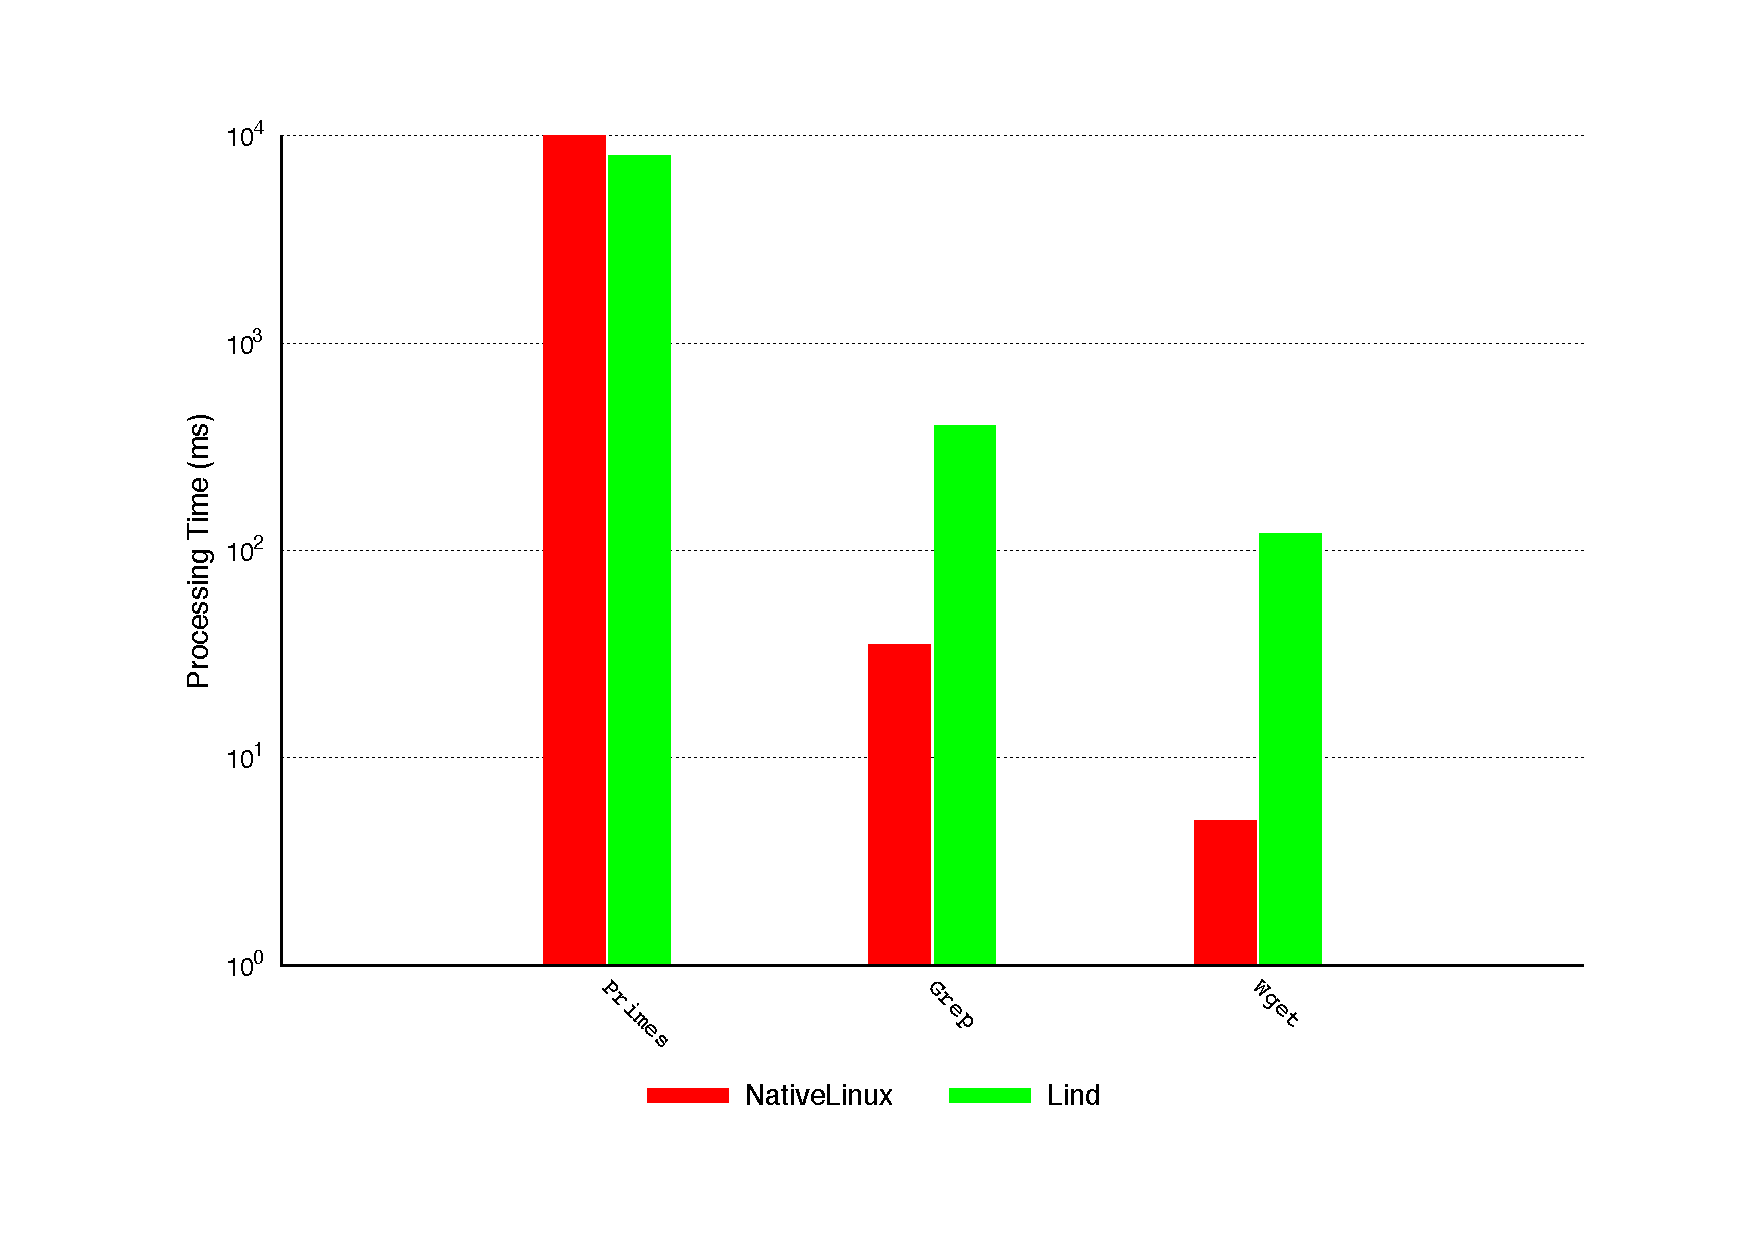
\includegraphics[width=1.6\columnwidth]{diagram/lind_oakland16_performance.pdf}
\caption{Applications Runtime Performance: Native Linux vs. Lind}
\label{fig:performance_applications}
\end{figure*}

Next, we ran the legacy application Tor in Lind. Tor runs unmodified in Lind. 
We used the benchmarks that come with Tor to test several of its common operations. 
A summary of the results is shown in Table \ref{table:performance_tor}. The benchmarks focus on cryptographic operations, 
which are CPU intensive, but also make syscalls like getpid, and reads to /dev/urandom.
Cell processing executes full packet encryption and decryption. In our test, 
Lind slowed these operations between 2.5x and 5x. We believe these slowdowns 
are caused by the differences in the code produced by NaCl, and the increased overhead from Lind system calls. 

As shown above,  Lind does incur some performance overhead in most cases. 
It should be noted though that, at this point, we have not  yet attempted to optimize its performance. 
It might be argued that, since an attack on the kernel can have devastating result, at this initial stage, 
a tradeoff between security and performance is justified. Despite this issue, 
the fact that Lind is able to run many legacy applications suggests that it is a positive step towards building new secure systems. 

\begin{table}
\centering
\scriptsize
\begin{tabular}{|r|r|r|r|}
  \hline
  Benchmark & Native Code & Lind & Impact  \\
  \hline
  Digest Tests: & & & \\
  Set & 54.80 nsec/element & 176.86 nsec/element & 3.22x \\
  Get & 42.30 nsec/element & 134.38 nsec/element & 3.17x \\
  Add & 11.69 nsec/element & 53.91 nsec/element & 4.61x \\
  IsIn & 8.24 nsec/element & 39.82 nsec/element & 4.83x \\
  \hline
  AES Tests: & & & \\
  1 Byte & 14.83 nsec/B & 36.93 nsec/B & 2.49x \\
  16 Byte & 7.45 nsec/B & 16.95 nsec/B & 2.28x \\
  1024 Byte & 6.91 nsec/B & 15.42 nsec/B & 2.23x \\
  4096 Byte & 6.96 nsec/B & 15.35 nsec/B & 2.21x \\
  8192 Byte & 6.94 nsec/B & 15.47 nsec/B & 2.23x \\
  Cell Sized & 6.81 nsec/B & 14.71 nsec/B & 2.16x \\
  \hline
  Cell Processing: & & & \\
  Inbound & 3378.18 nsec/cell & 8418.03 nsec/cell & 2.49x \\
  (per Byte) & 6.64 nsec/B & 16.54 nsec/B & - \\
  Outbound & 3384.01 nsec/cell & 8127.42 nsec/cell & 2.40x \\
  (per Byte) & 6.65 nsec/B & 15.97 nsec/B & - \\
  \hline
\end{tabular}
\caption{Performance Results on Tor's Built-in Benchmark Program: Native Linux vs. Lind }
\label{table:performance_tor}
\end{table}